\newpage
\texHeader

Now,\hypertarget{projectStructure tex}{} lets think about this whole text syntax. How exactly does it work? How will we be able to generate Java code from our simplified model code?

As you now know, Emoflon is a plug-in tool for Eclipse. More precisely, EMoflon needs the the Eclipse Modeling Framework (EMF) in order to work. EMF is comprised of two separate Metamodels - Genmodel and Ecore. The Genmodel contains the boring information about code generation like path and file information. 
We are more interested in Ecore, which we represent through our MOSL syntax. 

When you switched the project explorer from ``Projects" to ``Top Level Elements," you noticed that a few new nodes were created. Each node you see has a different criteria for grouping related Eclipse Projects together, which makes them your project ``Working Sets.'' The ``Specification'' node contains all the metamodels projects in a workspace (Fig. ~\ref{fig_modelSpecification}). That means, for every new Metamodel you create in your current workspace, all of the text code will be placed here. 

 \begin{figure}[htbp]
  \centering
  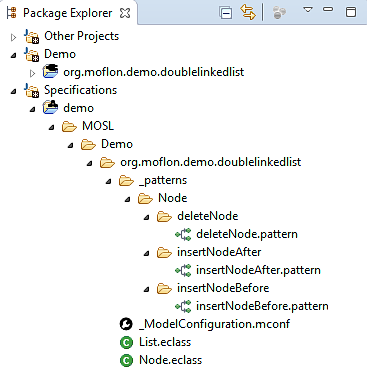
\includegraphics[width=0.5\textwidth]{eclipse_Specification}
  \caption{Eclipse: Specification Working Set}
  \label{fig_modelSpecification}
\end{figure}
  

Instead, lets look at the two eclass files and their syntax. Expand the folders, and you'll see that each eclass is declared in its own file. While you can combine several class delcarations in a single file in some languages (like Java), with MOSL it really is best to have them separated. It'll all make sense in a moment when we discuss Patterns.

Inspect the ``List'' class, and you'll see it has a just one EAttribute. EAttributes are defined by their name followed by a colon symbol and type.
This class also has a container reference represented by the diamond operator in front of an arrow.
The second reference type is a simple reference which
%
can be spotted in the next ``Node'' class. It's represented by just the arrow. EReferences name are immediately followed by their multiplicity % Include a reference to UML here if they need a refresher?
and then, just like an attribute, a colon and datatype.

While we're on the topic of syntax, lets have a quick overview on MOSL operators. The \texttt{`@'} before a name represents a bounded variable, \texttt{`--'} shows intended removal, and the opposite \texttt{`++'} operator signals something to be created. The destruction and creation operators can be placed before names or other operators, such as references.  All black items are elements of context, and must exist before and after the control flow. 

Lets go back to looking at the code. In the ``Node'' class, a few methods have been declared. You can see each function is remarkably small. In fact,the only thing the functions are doing are calling patterns. These patterns represent dynamic action within the program. Overall, the method and return statements are used just for control flow. A common format in a method like this would be {\texttt if (this) [pattern] else [pattern] }. The activities are never directly implemented. But where are these pattern files defined?

After many long discussions on correct control flow, it was decided that patterns must follow a strict, predictable path. Inspect Figure~\ref{fig_modelSpecification} again, and observe the locations where the patterns are stored. You'll notice that there is a folder for the ``Node'' class, and a folder for each method within that space. There's no folder for ``List'' purely because it never calls a pattern. It is imperative in the future that every pattern created follows this `Class/Method/patternName.pattern' set up. % Expand on this?? Seems to cut short

On a final note, one of the really neat things about references in MOSL is that the other object involved in the reference is automatically updated! Check out the ``DeleteNode'' pattern (Fig ~\ref{fig_MOSLOverview}). 

 \begin{figure}[htbp]
  \centering
  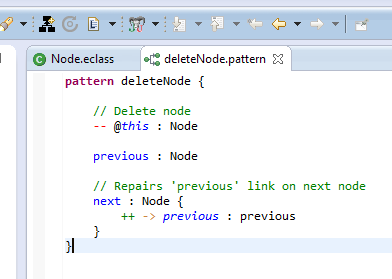
\includegraphics[width=0.6\textwidth]{MOSL_finalSyntaxReview}
  \caption{Eclipse/Ecore: The ``DeleteNode'' Pattern}
  \label{fig_MOSLOverview}
\end{figure}

% Forced next page to ensure footer lands in right place
\pagebreak
\fancyfoot[R]{  $\triangleright$ \hyperlink{codeGen common}{Next Step} }

You can see that a creation reference is made from Next to Previous, but the matching creation reference for Previous to Next is not. It's simply not needed! MOSL takes care of these automatically - you'll never have an issue with `hanging' links. It works for reference removal as well; You can see that there is a destroy command on {\texttt ``@this.''} It gets rid of the node, but it doesn't do anything about the previous and next references defined on it. That's because when the node is removed, everything attached to it will also be cleaned and updated.
 
So that's a quick overview of the MOSL language but again, how to we generate code from all of this?

First, eMoflon does not do a compelete code generation. Only the parser and error detection starts when you save files to improve performance. This means, to build the program, we need to press the ``Clean and Build'' from the eMoflon context menu when you right click on your working set. Alternatively, you can just press the ``Build'' icon beside the ``New Metamodel'' icon on the toolbar. 

Second, this is actually where Eclipse's EMF kicks in! Right when you save it! The .genmodel was automatically created - all we needed to make was the .ecore model. By invoking the ``Build" command above, code generation was initalized and completed. The subsection that follows offers a general code generation discussion, as it's virtually the same as it's visual counterpart.